\documentclass[mathserif]{beamer}%Agregar ,notes antes del ] para incluir las notas.
%~ \documentclass[handout]{beamer}

% Tema (colores, bordes, secciones, etc)
\usetheme{Warsaw}

% Configuracion del tema
\setbeamertemplate{navigation symbols}{} % saca los simbolos de abajo a la derecha
\useoutertheme{infolines} % muestra datos abajo de todo (nombre, numero de slide, etc)
\usecolortheme[RGB={72,123,127}]{structure}

% Paquetes usados
\usepackage[utf8]{inputenc}
\usepackage[spanish, es-tabla]{babel}
\usepackage{indentfirst}
\usepackage{beamerthemeshadow}
\usepackage{xspace}
\usepackage{latexsym}
\usepackage{ulem}
\usepackage{color}
\usepackage{tikz}
\usepackage{pgfplots}
\usepackage{colortbl, xcolor}
\usepackage{longtable}

\graphicspath{ {Images/} }

\newcommand{\tab}[1]{\hspace{.12\textwidth}\rlap{#1}}

\parskip=1ex

\title{Recolección online de grabaciones para el estudio de las variantes argentinas del español}
\author{Fernando Bugni}
\institute{Departamento de Computación - FCEyN - UBA}
\date{Fecha}

\begin{document}
	
\title{Recolección online de grabaciones para el estudio de las variantes argentinas del español}
\author{Fernando Bugni}
\institute{Departamento de Computación - Facultad de Ciencias Exactas - \\Universidad de Buenos Aires}
\date{2014}

\frame{\titlepage}

% % % % Introducción

\section{Introducción}
\begin{frame}
	\frametitle{Variantes del español en Argentina}
	\begin{figure}
		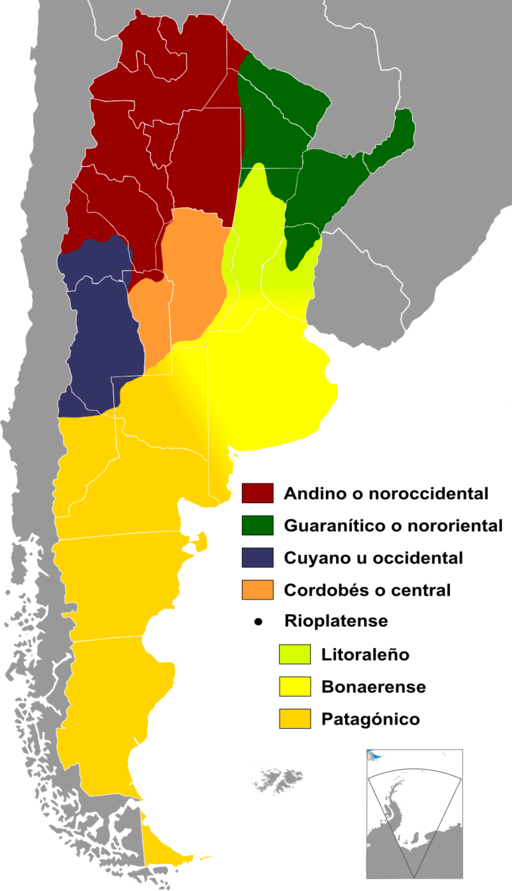
\includegraphics[scale=0.3]{../template_tesis/Images/Dialectos_del_idioma_espanol_en_Argentina.png}\\
	\end{figure}
\end{frame}

\begin{frame}
	\frametitle{Diferencias entre Córdoba y Buenos Aires}
		
	\begin{itemize}\itemsep=3ex
		\item \textbf{Regla 1: Los hablantes de Córdoba estiran la sílaba anterior a la acentuada mientras los de Buenos Aires no lo hacen} \\ 
	\end{itemize}	
	
	\begin{center}
		\textit{`Especta\textcolor{red}{\textbf{\textit{cu}}}\textcolor{blue}{lar}'}
	\end{center} 
	
	\tab{Sílaba acentuada en \textcolor{blue}{\textit{`-lar'}}} \\ 
	\tab{La sílaba anterior \textcolor{red}{\textit{`-cu-'}} se alarga para hablantes de Córdoba}
\end{frame}

\begin{frame}
	\frametitle{Diferencias entre Córdoba y Buenos Aires}
	\begin{itemize}\itemsep=3ex
		\item \textbf{Regla 2: Los hablantes de Córdoba aspiran y elisionan la /s/ al finalizar una palabra. Esto no sucede en Buenos Aires} \\ 
	\end{itemize}	
	
	\begin{center}
		\textit{`Pájaro\textcolor{red}{\textbf{\textit{s}}}'}
	\end{center} 
	
	\begin{center}
		/\textcolor{red}{\textbf{\textit{s}}}/ se acorta su duración en el hablante de Córdoba
	\end{center}
\end{frame}

\begin{frame}
 	\frametitle{Diferencias entre Córdoba y Buenos Aires}
 	\begin{itemize}\itemsep=3ex
 		\item \textbf{Regla 3: Para hablantes de Córdoba, la /s/ antes de la /c/ o /t/ suenan más suaves que para hablantes de Buenos Aires} \\ 
 	\end{itemize}
 	
 	\begin{center}
 		\textit{`Mo\textcolor{red}{s}ca'}
 	\end{center} 
 	
 	\begin{center}
 		/\textcolor{red}{s}/ suena más suave para Córdoba que para Buenos Aires
 	\end{center}
\end{frame}
 
\begin{frame}
 	\frametitle{Diferencias entre Córdoba y Buenos Aires}
 	\begin{itemize}\itemsep=3ex
 		\item \textbf{Regla 4: La `c' antes de la `t' se pronuncia con menor frecuencia para hablantes de Córdoba que para hablantes de Buenos Aires} \\ 
 	\end{itemize}
 	
 	\begin{center}
 		\textit{`Do\textcolor{red}{c}tor'}
 	\end{center} 
 	
 	\begin{center}
 		No debe sonar el fonema /\textcolor{red}{c}/
 	\end{center}
\end{frame}

\begin{frame}
	\frametitle{Diferencias entre Córdoba y Buenos Aires}
	\begin{itemize}\itemsep=3ex
		\item \textbf{Regla 5: Para hablantes cordobeces la `y’ y `ll’ se pasa a `i’. No sucede esto para Buenos Aires} \\ 
	\end{itemize}
	
	\begin{center}
		\textit{`\textcolor{red}{ll}uvia'}
	\end{center} 
	
	\begin{center}
		Palabras con el fonema /\textcolor{red}{y}/ o /\textcolor{red}{ll}/ se pronuncian /\textcolor{red}{j}/
	\end{center}
\end{frame}
 
\begin{frame}
	\frametitle{Diferencias entre Córdoba y Buenos Aires}
	\begin{itemize}\itemsep=3ex
		\item \textbf{Regla 6: En hablantes cordobeces la /r/ no vibra mientras que en Buenos Aires pasa lo contrario} \\ 
	\end{itemize}	
	
	\begin{center}
		\textit{`Espá\textcolor{red}{rr}ago'}
	\end{center} 
	
	\begin{center}
		Para Córdoba /\textcolor{red}{r}/ debe ser suave en comparación de Buenos Aires
	\end{center}
\end{frame} 

% % % % Diseño del experimento
\begin{frame}
	\frametitle{Diseño del experimento}
	\begin{itemize}\itemsep=10ex
		\item \textbf{Frases Comúnes}: habla espontánea
		\item \textbf{Frases Amper}: reconocer palabra acentuada
	\end{itemize}	
\end{frame} 

\begin{frame}
	\frametitle{Diseño del experimento}
	{\Large Frases Comúnes} \\
	Pronunciar frases popularmente conocidas
	
	\begin{itemize}
		\item Objetivo: pronunciación espontánea
		\item Reglas a cubrir: 2 a 6
	\end{itemize}
\end{frame} 

\begin{frame}
	\frametitle{Diseño del experimento}
	\begin{center}
		\textbf{`En la pelea se conoce al soldado,} \\ 
		\textbf{sólo en la \textcolor{red}{victoria} se conoce al \textcolor{red}{caballero}’}
	\end{center}
	
	\begin{itemize}
		\item \textcolor{red}{\textbf{`victoria’}} cubre la regla 4 que nos propone medir la duración de la \textit{/c/} antes de la \textit{/t/}. 
		\item \textcolor{red}{\textbf{`caballero’}} para la regla 5: el fonema \textit{/ll/} se pasa a \textit{/i/} 
	\end{itemize}	
\end{frame} 

%\begin{frame}
%	\frametitle{Diseño del experimento}
%	\scriptsize
%	\begin{longtable}{| p{0.3\textwidth} || p{0.15\textwidth} | p{0.15\textwidth} | p{0.15\textwidth} | p{0.15\textwidth}| p{0.15\textwidth} | } 
%		\hline
%		\textbf{Frase} & \textbf{2 - Aspiración y elisión de /s/} & \textbf{3 - La 's' antes de la 'c' o 't' no suenan} & \textbf{4 - La 'c' antes de la 't' no suenan}& \textbf{5 - La 'y' y 'll' se pasa a 'i'} & \textbf{6 - La 'r' no debe sonar} \\ \hline	
%		
%		
%		'No hay dos sin tres' & dos, tres & & & & \\ \hline
%		'Más difícil que encontrar una aguja en un pajar' & más &&&& \\ \hline
%		'Más perdido que turco en la neblina' & más &&&&  \\ \hline
%		'No le busques la quinta pata al gato' & busques & busques &&&  \\ \hline
%		%	'Todo bicho que camina va al asador' &  \\ \hline
%		%	'Caminante no hay camino se hace camino al andar' &  \\ \hline
%		'Se te escapó la tortuga' && escapó &&&  \\ \hline
%		'Todos los caminos conducen a Roma' & todos, los, caminos &&&&  \\ \hline
%		'No hay mal que dure cien anos' & años &&&& \\ \hline
%		'Siempre que llovió paro' &&&& llovió & \\ \hline
%		'Cría cuervos que te sacaran los ojos' & cuervos, los, ojos &&&&  \\ \hline
%		'La tercera es la vencida' & es &&&& \\ \hline
%		'Calavera no chilla' &&&& chilla &  \\ \hline
%		'La gota que rebalsó el vaso' &&&&& rebasó \\ \hline
%		'La suegra y el doctor cuanto más lejos mejor' & más, lejos & doctor&&& \\ \hline
%		'A la mujer picaresca cualquiera la pesca' && picaresca &&&  \\ \hline
%		'Quien siembra vientos recoge tempestades' & vientos &&&& recoge  \\ \hline
%		%	'Un grano no hace granero pero ayuda a su compañero' & \\ \hline
%		'La arquitectura es el arte de organizar el espacio' & es && arquitectura && \\ \hline
%		'El amor actúa con el corazón y no con la cabeza' &&& actúa&& \\ \hline
%		'No dudes actúa' &&& actúa&&  \\ \hline
%		%	'El niño es realista; el muchacho, idealista; el hombre, escéptico, y el viejo místico' &  \\ \hline
%		'Perro que ladra no muerde' &&&&& perro \\ \hline
%		'La musica es sinónimo de libertad, de tocar lo que quieras y como quieras' & es, quieras &&&& \\ \hline
%		'La belleza que atrae rara vez coincide con la belleza que enamora' &&&& belleza & \\ \hline
%		'No esta mal ser bella lo que esta mal es la obligación de serlo' &&&& bella & \\ \hline
%		'La batalla más difícil la tengo todos los días conmigo mismo' & más &&& batalla & \\ \hline
%		'El que no llora no mama' &&&& llora & \\ \hline
%		'En la pelea se conoce al soldado solo en la victoria se conoce al caballero' &&& victoria & caballero &\\ \hline
%		'La lectura es a la mente lo que el ejercicio al cuerpo' & es && lectura &&  \\ \hline
%		'El pez por la boca muere' & pez &&&& \\ \hline
%		'En boca cerrada no entran moscas' & moscas & moscas &&& cerrada  \\ \hline
%		'Más vale pájaro en mano que cien volando' & más &&&& \\ \hline
%		%	'La curiosidad mató al gato' &  \\ \hline
%		'Río revuelto ganancia de pescadores' & pescadores & pescadores &&& río, revuelto  \\ \hline
%		'No hay que pedirle peras al olmo' & peras &&&& \\ \hline
%		
%		\caption{Frases conocidas} 
%		\label{fig22tabla}
%		\end{longtable}
%\end{frame}

\begin{frame}
\frametitle{Diseño del experimento}
	{\Large Frases Amper} \\
	Pronunciar frases con una estructura fija variando acentuaciones
	
	\begin{itemize}
		\item Objetivo: cubrir acentuaciones
		\item Regla a cubrir: 1
	\end{itemize}
	
{\footnotesize 	
	\begin{center}
		\textit{Sujeto+`` salió ’’+Adjetivo} 
	
		\begin{itemize}
			\item Sujeto: \textit{``El canapé’’, ``El repollo’’, ``El espárrago’’}.
			\item Adjetivo: \textit{``espectacular’’, ``delicioso’’, ``riquísimo’’}.
		\end{itemize}
		
	\end{center}
}
\end{frame} 

\begin{frame}
	\frametitle{Diseño del experimento}

	\begin{center}
		\textbf{``El \textcolor{red}{canapé} salió \textcolor{red}{delicioso}’’}
	\end{center}
	
	\begin{itemize}
		\item Canapé: palabra aguda
		\item Delicioso: palabra grave
	\end{itemize}
\end{frame} 

%\begin{frame}
%	\frametitle{Frases Amper}
%	
%	\small 
%	\begin{center}
%		\begin{longtable}{| p{0.15\textwidth} | p{0.08\textwidth} | p{0.15\textwidth} || p{0.15\textwidth} | p{0.12\textwidth} | p{0.15\textwidth} |} 
%		\hline
%		%\multicolumn{6}{| p{0.9\textwidth} |} {\textbf{1 - Localice la sílaba acentuada en la palabra y estirar la sílaba anterior}} \\ \hline
%		\multicolumn{3}{| p{0.45\textwidth} ||}{Frase} & \textbf{Aguda} & \textbf{Grave} & \textbf{Esdrújula} \\ \hline 
%		\textit{El canapé} & \textit{salió} & \textit{espectacular} & espectacular, canapé & & \\ \hline
%		\textit{El canapé} & \textit{salió} & \textit{delicioso} & canapé & delicioso & \\ \hline
%		\textit{El canapé} & \textit{salió} & \textit{riquísimo} & canapé & & riquísimo \\ \hline
%		\textit{El repollo} & \textit{salió} & \textit{espectacular} & espectacular & repollo & \\ \hline
%		\textit{El repollo} & \textit{salió} & \textit{delicioso} &  & repollo, delicioso & \\ \hline	
%		\textit{El repollo} & \textit{salió} & \textit{riquísimo} & & repollo & riquísimo \\ \hline
%		\textit{El espárrago} & \textit{salió} & \textit{espectacular} & espectacular & & \\ \hline
%		\textit{El espárrago} & \textit{salió} & \textit{delicioso} & & delicioso & \\ \hline
%		\textit{El espárrago} & \textit{salió} & \textit{riquísimo} & & & riquísimo \\ \hline	
%		
%		\caption{Frases AMPER} 
%		\label{fig21table}
%	\end{longtable}
%	\end{center}
%\end{frame}

\begin{frame}
	\frametitle{Diseño del experimento}
	
	\Large{Trazas: combinación de frases}
	
	\begin{center}
		\begin{tikzpicture}
			%1-3 comun 4 amper 5-6 comun 6 amper 7-9 comun
			%10 amper 11-13 comun 14 amper
			%\fill[red!20](0,0) rectangle (0.4,0.4); 
			%\fill[blue!20!white](0.4,0) rectangle (0.8,0.4); 
			\fill[blue!20!white](0,0) rectangle (0.4*3,0.4);
			\fill[red!20](0.4*3,0) rectangle (0.4*5,0.4); 
			\fill[blue!20!white](0.4*5,0) rectangle (0.4*7,0.4);
			\fill[red!20](0.4*7,0) rectangle (0.4*8,0.4); 
			\fill[blue!20!white](0.4*8,0) rectangle (0.4*10,0.4);
			\fill[red!20](0.4*10,0) rectangle (0.4*11,0.4);
			\fill[blue!20!white](0.4*11,0) rectangle (0.4*13,0.4);
			\fill[red!20](0.4*13,0) rectangle (0.4*14,0.4);
			\fill[blue!20!white](0.4*14,0) rectangle (0.4*16,0.4);
			\fill[red!20](0.4*16,0) rectangle (0.4*17,0.4);			
			\fill[blue!20!white](0.4*17,0) rectangle (0.4*19,0.4);
			\fill[red!20](0.4*19,0) rectangle (0.4*20,0.4);			
			\fill[blue!20!white](0.4*20,0) rectangle (0.4*22,0.4);
			\fill[red!20](0.4*22,0) rectangle (0.4*24,0.4);			
			\fill[blue!20!white](0.4*24,0) rectangle (0.4*25,0.4);
			
			\draw[step=0.4cm,very thin,fill=blue!20!white] (0,0) grid (10,0.4);
			
		\end{tikzpicture}
		
		\begin{itemize}
			\item[] 
				\begin{tikzpicture}
					\draw[step=0.4cm,very thin,fill=blue!20!white] (0,0) grid (0.4,0.4) rectangle (0,0);
				\end{tikzpicture} Frases comúnes
			\item[] 
			\begin{tikzpicture}
			\draw[step=0.4cm,very thin,fill=red!20] (0,0) grid (0.4,0.4) rectangle (0,0);
			\end{tikzpicture} Frases Amper				
		\end{itemize}
		
		\begin{center}
			Intercalado: 1 ó 3 Frases comúnes cada una Amper
		\end{center}
	\end{center}
	
\end{frame}

\begin{frame}
	\frametitle{Diseño del experimento}
	
	\begin{figure}[H]
		\centering
		\begin{tikzpicture}
		\begin{axis}[
		width=8cm,
		height=6cm,
		title={Porcentaje del total de frases por regla},
		xlabel={Cantidad de grabaciones},
		ylabel={Porcentaje del total de frases},
		xmin=0, xmax=25,
		ymin=0, ymax=100,
		xtick={0,5,10,15,20,25,30},
		ytick={0, 25, 50, 75, 100},
		%legend pos=south east,
		ymajorgrids=true,
		xmajorgrids=true,
		grid style=dashed
		] 
		
		\addplot [mark=times*, line width=0.5pt]
		coordinates {
			(0,0)(1, 0)(2, 5)(3, 11)(4, 17)(5, 17)(6, 23)(7, 29)(8, 35)(9, 41)(10, 41)(11, 47)(12, 52)(13, 52)(14, 52)(15,58)(16, 64)(17, 64)(18, 70)(19, 76)(20, 76)(21, 76)(22, 82)(23, 82)(24, 88)(25, 94)(26, 100)
		};\addlegendentry{Regla 2};
		
		\addplot [mark=times*, dash pattern=on 10pt off 5pt, line width=0.5pt]
		coordinates {
			(0,0)(1,0)(2,0)(3,25)(4,25)(5,25)(6,25)(7,25)(8,50)(9,50)(10,50)(11,50)(12,50)(13,75)(14,75)(15,75)(16,75)(17,75)(18,75)(19,75)(20,100)(21,100)(22,100)(23,100)(24,100)(25,100)(26,100)
		};\addlegendentry{Regla 3};
		
		\addplot [mark=times*, line width=2pt] 
		coordinates {
			(0,0)(1, 0)(2, 0)(3, 0)(4, 25)(5, 25)(6, 50)(7, 50)(8, 50)(9, 75)(10, 75)(11, 75)(12, 75)(13, 75)(14, 75)(15,75)(16, 75)(17, 75)(18, 75)(19, 75)(20, 75)(21, 100)(22, 100)(23, 100)(24,100)(25,100)(26, 100)
		};\addlegendentry{Regla 4};
		
		\addplot [mark=times*, dash pattern=on 10pt off 5pt, line width=2pt]
		coordinates {
			(0,0)(4,0)(5,50)(13,50)(14,100)(26,100) 
		};\addlegendentry{Regla 5};
		
		\addplot [mark=times*, dotted, line width=2pt] 
		coordinates {
			(0,0)(2,20)(6,20)(7,40)(9,40)(10,60)(16,60)(17,80)(22,80)(23,100) 
		};\addlegendentry{Regla 6};
		
		
		%%		Tarea	rule 2:	rule 3:	rule 4:	rule 5:	rule 6:
		%		1	0	0	0	0	0
		%		2	5	0	0	0	20
		%		3	11	25	0	0	20
		%		4	17	25	25	0	20
		%		5	17	25	25	50	20
		%		6	23	25	50	50	20
		%		7	29	25	50	50	40
		%		8	35	50	50	50	40
		%		9	41	50	75	50	40
		%		10	41	50	75	50	60
		%		11	47	50	75	50	60
		%		12	52	50	75	50	60
		%		13	52	75	75	50	60
		%		14	52	75	75	100	60
		%		15	58	75	75	100	60
		%		16	64	75	75	100	60
		%		17	64	75	75	100	80
		%		18	70	75	75	100	80
		%		19	76	75	75	100	80
		%		20	76	100	75	100	80
		%		21	76	100	100	100	80
		%		22	82	100	100	100	80
		%		23	82	100	100	100	100
		%		24	88	100	100	100	100
		%		25	94	100	100	100	100
		%		26	100	100	100	100	100
		
		\end{axis}
		\end{tikzpicture}
		\caption{Porcentaje del total de frases grabadas por cada regla}
		\label{figFracesTraza}
	\end{figure}
\end{frame}


\begin{frame}
	\frametitle{Sistema de grabación online}
	
	\begin{figure}[h!]
		\centerline{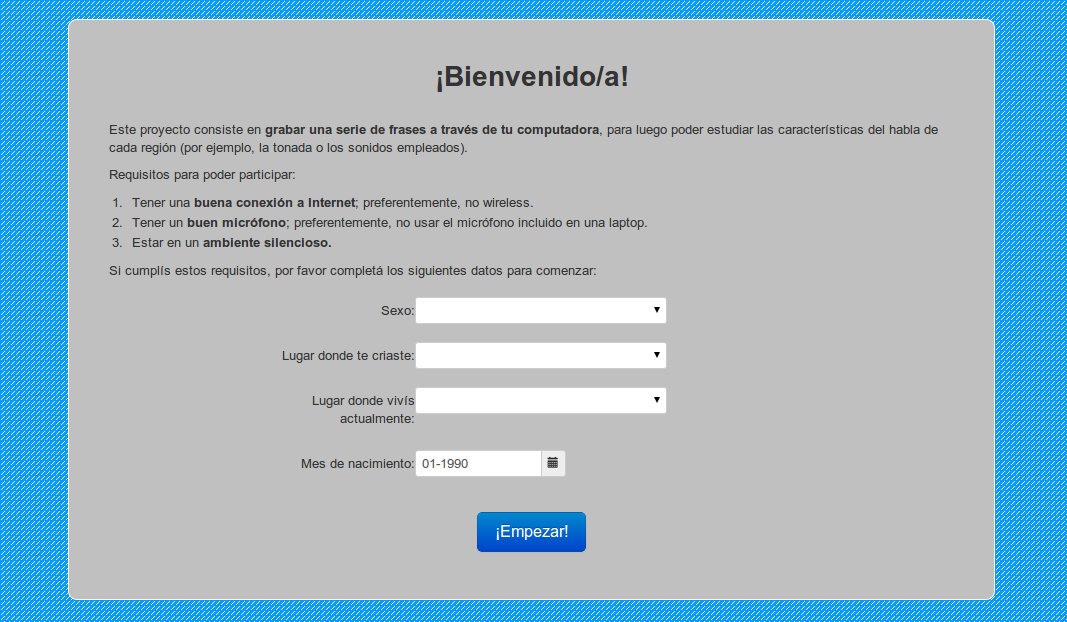
\includegraphics[width=0.8\textwidth]{pag-inicio2} }
		\caption{Encuesta inicial del sistema}
		\label{figEncuesta}
	\end{figure}
\end{frame}

%\begin{frame}
%	\frametitle{Sistema de grabación online}
%	
%	\begin{figure}[h!]
%		\centerline{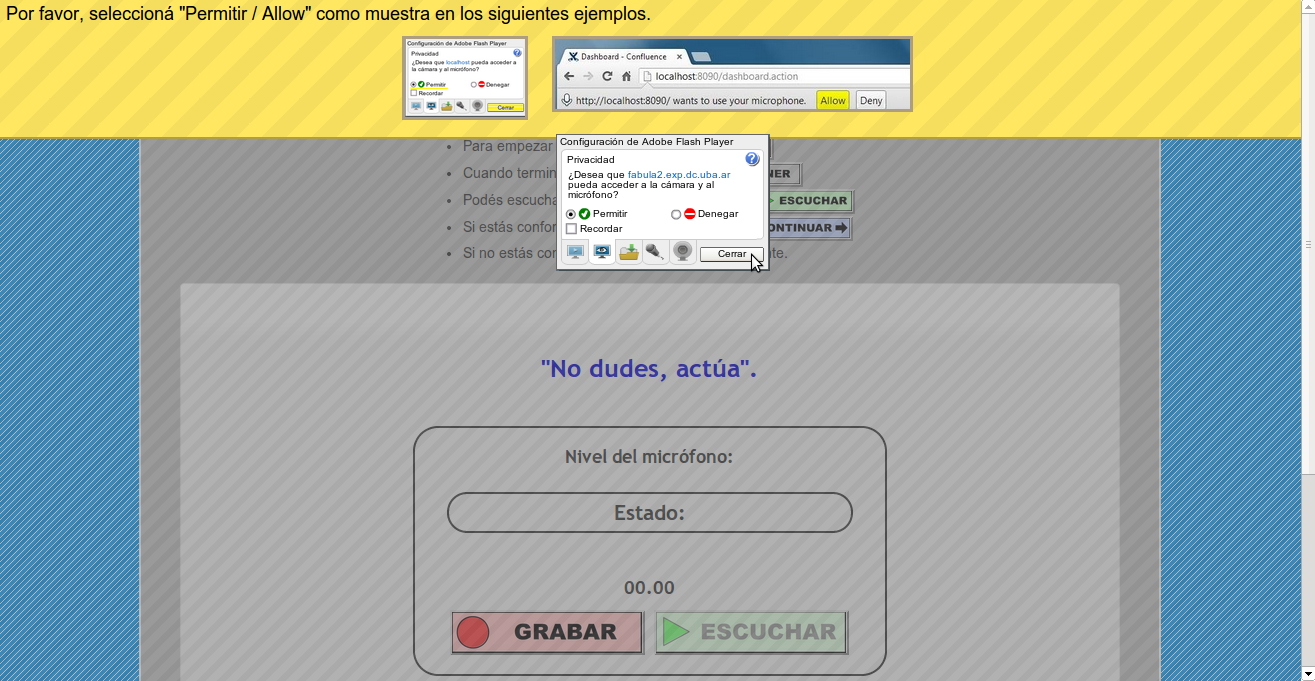
\includegraphics[width=0.8\textwidth]{pag-allow1} }
%		\caption{Habilitar micrófono}
%		\label{figEncuesta}
%	\end{figure}
%\end{frame}

\begin{frame}
	\frametitle{Sistema de grabación online}
	
	\begin{figure}[h!]
		\centerline{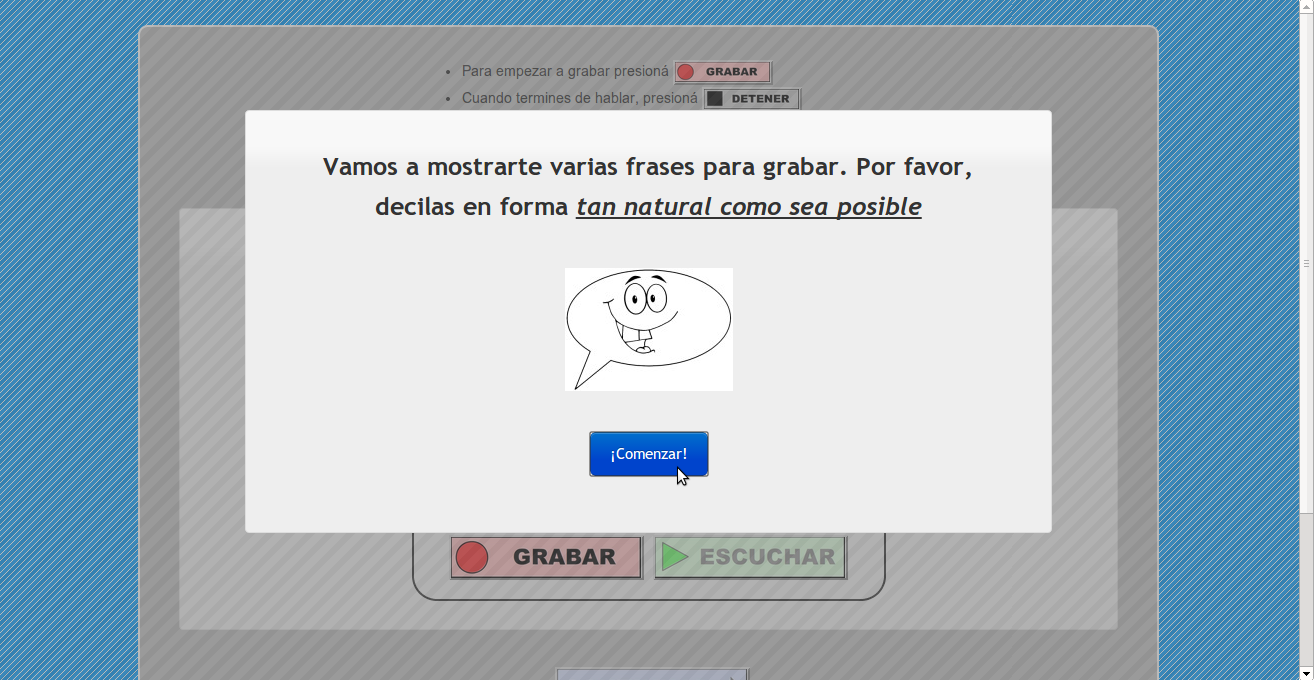
\includegraphics[width=0.8\textwidth]{pag-info2} }
		\caption{Explicación del experimento}
		\label{figEncuesta}
	\end{figure}
\end{frame}

\begin{frame}
	\frametitle{Sistema de grabación online}
	
	\begin{figure}[h!]
		\centerline{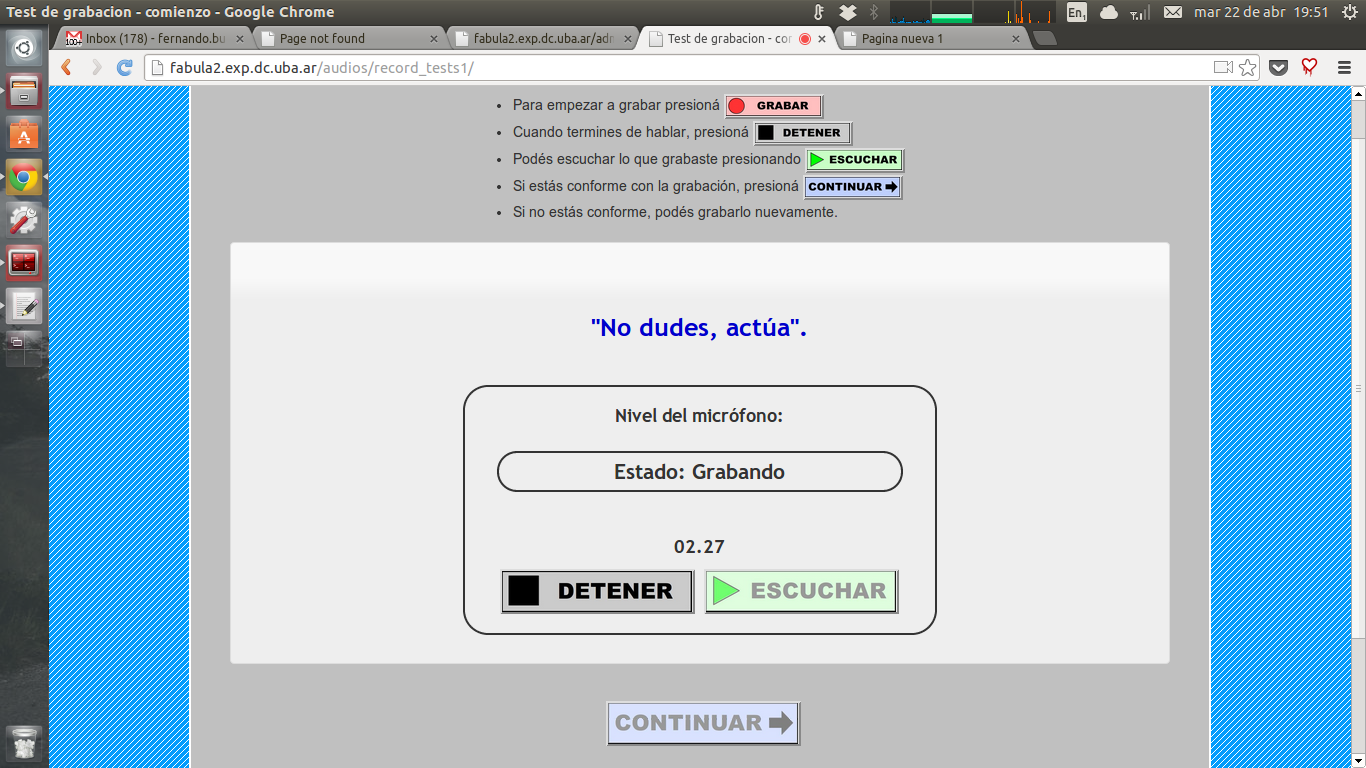
\includegraphics[width=0.8\textwidth]{pag-grabar1} }
		\caption{Grabando}
		\label{figEncuesta}
	\end{figure}
\end{frame}

\begin{frame}
	\frametitle{Sistema de grabación online}
	
	\begin{figure}[h!]
		\centerline{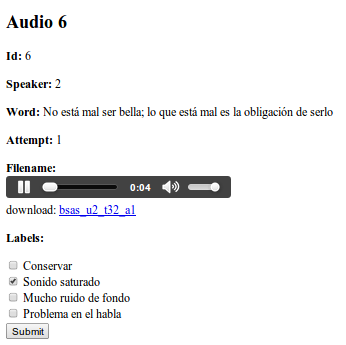
\includegraphics[width=0.6\textwidth]{categorizando_audios} }
		\caption{Administrador}
		\label{figEncuesta}
	\end{figure}
\end{frame}

\begin{frame}
	\frametitle{Datos obtenidos}
	
	\begin{table}[h]
		\centering
		\begin{tabular}{|l|c|c|c|c|}
			\hline
			\textbf{}  & \textbf{Bs.As. } & \textbf{Cba.} & \textbf{Total} \\ \hline
			%\textbf{Conservar}  & 222 & 105 & 327 \\ \hline
			\textbf{Conservar}  & 220 & 90 & 310 \\ \hline
			\textbf{Problemas en el habla}  & 33 & 15 & 48 \\ \hline
			\textbf{Mucho ruido de fondo}  & 2 & 12 & 14 \\ \hline
			\textbf{Sonido saturado}  & 2 & 0 & 2 \\ \hline
		\end{tabular}
		\caption{Evaluación manual de las grabaciones}
		\label{eva_table}
	\end{table}
	
	\begin{table}[H]
		\centering
		\begin{tabular}{|l|c|c|c|}
			\hline
			\textbf{}  & \textbf{Bs.As. } & \textbf{Cba.} & \textbf{Total} \\ \hline
			\textbf{Todos los intentos}  & 220 & 90 & 310 \\ \hline
			\cellcolor{blue!25}\textbf{Último intento}  & \cellcolor{blue!25}\textbf{181} & \cellcolor{blue!25}\textbf{79} & \cellcolor{blue!25}\textbf{260} \\ \hline
		\end{tabular}
		\caption{Cantidad de audios repetidos}
		\label{eva_table_rep}
	\end{table}
\end{frame}

\begin{frame}
	\frametitle{Extracción de información}
	
	\begin{center}
		\begin{itemize}
			\item ProsodyLab
			\item Python 2.7, SciPy y Numpy
			\item Pymatlab 
		\end{itemize}
	\end{center}
	
	\begin{figure}[h!]
		\centerline{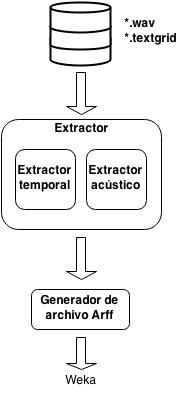
\includegraphics[width=0.4\textwidth]{diagrama_workflow} }
	\end{figure}
\end{frame}


\begin{frame}
	\frametitle{Extracción de información}
	
	\begin{figure}[h!]
		\centerline{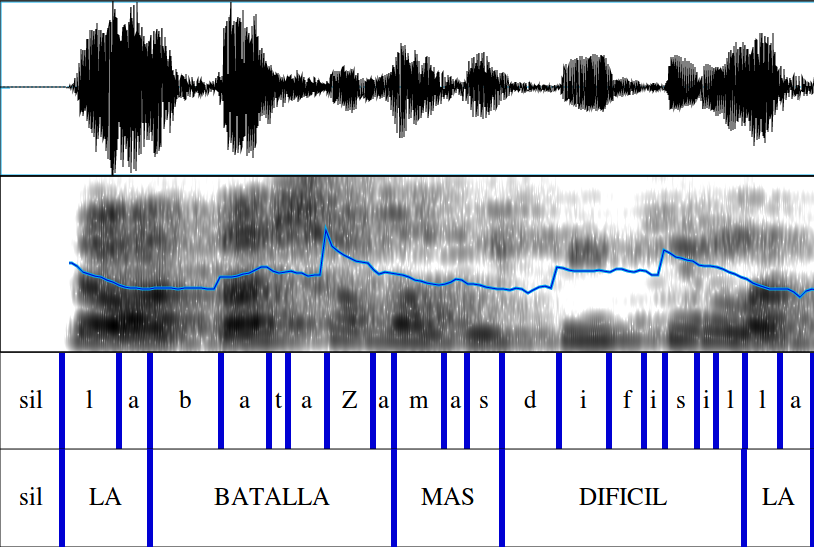
\includegraphics[width=0.9\textwidth]{espectograma_u3_t33_a1} }
	\end{figure}
\end{frame}

\begin{frame}
	\frametitle{Extracción de información}
	\Large {Atributos fonéticos}
	
	\begin{itemize}
		\item Duración de 'kt'
		\item Duración de 'sc'
		\item Duración de 'll'
		\item Duración de 'rr'
		\item Duración de 's' final
		\item Duración de cada fonema
		\item Duración de cada vocal 
		\item Duración de cada consonante
	\end{itemize}
\end{frame}


\begin{frame}
	\frametitle{Extracción de información}
	\Large {Atributos fonético: cálculo duración de `kt’}
	
	\begin{center}
		{\textbf{\textit{``en la pelea se konose al soldaDo solo en la biktorja se konose al kaBaZero’’}}}
	\end{center}
	
	\begin{figure}[H]
		\centering
		\begin{tikzpicture}[xscale=0.5]
		\draw[x=2cm,step=0.05pt,thick,>=latex](0,0) -- (7.5,0);
		\foreach \Xc in {0,...,15}
		{
			\draw[thick] 
			(\Xc,0) -- ++(0,05pt);
		}
		\draw[dotted,thick] (-0.5,0) -- (0,0);
		\draw[dotted,thick] (15,0) -- (15.5,0);
		% la victoria se conoce
		\foreach \Xc/\Texto in 
		{5/k}
		{
			\fill[black] 
			([xshift=2pt]\Xc,0.05)  
			rectangle node[above] {\strut\small\Texto} 
			([xshift=-2pt]\Xc+1,0.15);  
		}
		\foreach \Xc/\Texto in 
		{0/l,1/a,2/$sil$,3/b,4/i,6/t,7/o,8/r,9/j,10/a,11/$sil$,12/s, 13/e, 14/$sil$}
		{
			\node[above] at ([xshift=15pt]\Xc,0.05){\strut\small\Texto} ;
		}
		\end{tikzpicture}
	\end{figure}
	
	\normalsize 
	\hspace{1cm} \[\frac{ X - \mu }{ \sigma }\]
	
	\begin{itemize}
		\item $X$ es el valor a normalizar (por ej.: la duración de un fonema dado).
		\item $\mu$ es el promedio de duración de la unidad utilizada en la grabación.
		\item $\sigma$ es el desvío estándar de la unidad utilizada en la grabación.
	\end{itemize}
	
\end{frame}


\begin{frame}
	\frametitle{Extracción de información}
	\Large {Atributos silábicos}
		
	\begin{itemize}
		\item Duración de la sílaba acentuada
		\item Duración de la sílaba anterior a la acentuada
	\end{itemize}
\end{frame}


\begin{frame}
	\frametitle{Extracción de información}
	\Large {Atributos silábico: cálculo duración de `kt’}

	\begin{center}
		{\textbf{\textit{``en la pelea se konose al soldaDo solo en la biktorja se konose al kaBaZero’’}}}
	\end{center}

	\begin{figure}[H]
		\centering
		\begin{tikzpicture}[xscale=0.7]
		\draw[x=2cm,step=0.05cm,thick,>=latex](0,0) -- (7.5,0);
		\foreach \Xc in {0,...,15}
		{
			\draw[thick] 
			(\Xc,0) -- ++(0,05pt);
		}
		\draw[dotted,thick] (-0.5,0) -- (0,0);
		\draw[dotted,thick] (15,0) -- (15.5,0);
		% la victoria se conoce
		\foreach \Xc/\Texto in 
		{2/bik,8/ko}
		{
			\fill[black] 
			([xshift=2pt]\Xc,0.05)  
			rectangle node[above] {\strut\small\Texto} 
			([xshift=-2pt]\Xc+1,0.15);  
		}
		\foreach \Xc/\Texto in 
		{0/la,1/$sil$,3/to*,4/rja,5/$sil$,6/se,7/$sil$,9/no*,10/se,11/$sil$,12/al, 13/$sil$, 14/ka}
		{
			\node[above] at ([xshift=15pt]\Xc,0.05){\strut\small\Texto} ;
		}
		\end{tikzpicture}
	\end{figure}
	
	\normalsize 
	\hspace{1cm} \[\frac{ X - \mu }{ \sigma }\]
	
	\begin{itemize}
		\item $X$ es el valor a normalizar (por ej.: la duración de un fonema dado).
		\item $\mu$ es el promedio de duración de la unidad utilizada en la grabación.
		\item $\sigma$ es el desvío estándar de la unidad utilizada en la grabación.
	\end{itemize}
	
\end{frame}

\begin{frame}
	\frametitle{Análisis}
	\Large {Clasificadores}
	\begin{itemize}
		\item Zero rules
		\item RIPPER
		\item C4.5
		\item Support vectors machines
		\item Naive Bayes
	\end{itemize}
\end{frame}

\begin{frame}
	\frametitle{Análisis}
	\Large {Cross-validations}
	\begin{itemize}
		\item Grupos de hablantes
		\item Dejando un hablante fuera promediando los atributos
		\item Dejando un hablante fuera promediando los atributos desconocidos
	\end{itemize}
\end{frame}

\begin{frame}
\frametitle{Compuertas - AND}
\begin{figure}
\begin{tabular}{cc|c}
A & B & A AND B \\
\hline
0 & 0 & 0\\
0 & 1 & 0\\
1 & 0 & 0\\
1 & 1 & 1
\end{tabular}
\end{figure}
\end{frame}

% % %


\end{document}

%
%\begin{frame}
%	\frametitle{Compuertas - datasheet}
%	\begin{figure}
%		\includegraphics[scale=0.4]{datasheetDM7408N.png}\\
%	\end{figure}
%\end{frame}

%\begin{frame}
%	\frametitle{Propiedades}
%	\begin{center}
%	\begin{footnotesize}
%	\begin{tabular}[h]{|c|c|c|}
%	\hline
%	Identidad & $1.A=A$                      &     $0+A=A$            \\
%	 Nulo            &      $0.A=0$                      &     $1+A=1$            \\
%	 Idempotencia    &       $A.A=A$                      &     $A+A=A$            \\      
%	 Inverso         &       $A.\overline{A}=0$           &     $A+\overline{A}=1$ \\      
%	 Conmutatividad  &       $A.B=B.A$                    &     $A+B=B+A$          \\
%	 Asociatividad   &       $(A.B).C=A.(B.C)$            &     $(A+B)+C=A+(B+C)$  \\
%	 Distributividad &      $A+(B.C) = (A+B).(A+C)$      &     $A.(B+C)=A.B+A.C$  \\
%	 Absorci\'on     &       $A.(A+B)=A$                  &     $A+A.B = A$        \\
%	 De Morgan       &  $\overline{A.B} = \overline{A} + \overline{B}$ & $\overline{A+B} = \overline{A} . \overline{B}$ \\
%	\hline
%	\end{tabular}\\
%	\end{footnotesize}
%	\end{center}
%\end{frame}


%\begin{frame}
%\frametitle{M\'as circuitos combinatorios!}
%\pause			
%\underline{Decodificador de n bits:} Tiene n entradas y $2^n$ salidas. Sea k el n\'umero representado en binario en la entrada del decodificador, la salida $e_k$ tendr\'a un uno l\'ogico, mientras que para todas las dem\'as se\~nales de salida habr\'a un cero l\'ogico.\\
%\pause
%\underline{Codificador de n bits:} Tiene n entradas y $log_2(n)$ salidas. En la salida muestra en binario el n\'umero de la entrada que esta levantada, de haber mas de una o ninguna, el comportamiento del circuito depender\'a de la implementaci\'on del fabricante.\\
%\pause
%\underline{Multiplexor de n entradas:} Tienen n entradas, una salida y $log_2(n)$ se\~nales de control. Mediante las se\~nales de control se indica cual entrada es requerida en la salida.\\
%\pause
%\underline{Demultiplexor de n salidas:} Tienen n salidas, una entrada y $log_2(n)$ se\~nales de control. Igual que el multiplexor, pero elijo mediante las se\~nales de control por cual se\~nal de salida muestro la entrada.
%\end{frame}
%
%\begin{frame}
%\frametitle{La práctica...}
%\begin{center}
%Con lo visto hoy pueden realizar hasta\\ el ejercicio 13 de la práctica 2.
%
%Bibliograf\'ia recomendada: The Essentials of Computer Organization and Architecture - Linda Null
%- Cap\'itulo 3
%\end{center}
%\end{frame}